\section{Numerical Implementation}
\label{sec:methods}

\subsection{Finite element discretisation}
\label{sec:fem}
All partial differential equations are solved with FEniCSx
(DOLFINx~v0.7.3)~\cite{fenicsx2022} on structured triangular meshes.
The primary mesh uses $80\times20$ elements
(1600 elements, $\Delta x = \Delta y = 25\,\mu$m);
a coarser $20\times5$ mesh is used for rapid parameter screening.

The Brinkman equations~\eqref{eq:brinkman} are discretised with the
inf-sup stable Taylor--Hood element pair: continuous piecewise quadratic
velocities (P2) and continuous piecewise linear pressure (P1), giving
approximately 20\,000 velocity degrees of freedom on the $80\times20$ mesh.
The convection--diffusion equation~\eqref{eq:convdiff} and its
adjoint~\eqref{eq:adj_conc} are discretised with continuous piecewise
linear elements (P1) and stabilised using the SUPG method~\cite{donea2003}.
The design variable $\rho$ and the filtered and projected fields
$\tilde\rho$, $\bar\rho$ are also discretised with P1 elements.
Weak forms are assembled using the Unified Form Language (UFL);
all integrals are evaluated with exact quadrature.

\subsection{Linear solvers}
All linear systems arising from the forward and adjoint Brinkman problems
are solved with a direct LU factorisation (MUMPS) via PETSc's
\texttt{preonly}/\texttt{lu} combination.
This choice provides robust, parameter-free solutions for the moderate
meshes used here ($\lesssim 30\,000$ degrees of freedom).
For larger-scale problems, an iterative solver is available: a
block-triangular field-split preconditioner with algebraic multigrid
(HYPRE) for the velocity block and the pressure Schur
complement~\cite{elman2014}; scalability results are in
Supplementary Information~S1.

\subsection{Optimisation algorithm}
The design is updated using the Optimality Criteria (OC)
method~\cite{bendsoe2003} as the default:
\begin{equation}
    \rho^{\mathrm{new}} = \max\!\bigl(\rho_{\min},\,
        \min(\rho_{\max},\,\rho^{\mathrm{old}} \cdot B^\eta)\bigr),
    \qquad B = -\frac{\mathrm{d}J/\mathrm{d}\rho}{\Lambda},
    \label{eq:oc}
\end{equation}
with damping exponent $\eta=0.5$ and move limit $0.15$.
An optional hybrid schedule (OC for iterations~0--299,
MMA~\cite{svanberg1987} for iterations~300--599) is also
implemented and documented in Table~\ref{tab:mma_comparison},
but is not the default configuration.
The volume constraint is enforced explicitly in both update rules
via Lagrange multiplier bisection (OC) and dual bisection (MMA).

\subsection{Default configuration and continuation settings}
\label{sec:continuation}
Each component of the continuation schedule is documented
in Table~\ref{tab:continuation} with its motivation.
The hybrid OC/MMA schedule is validated by direct comparison:
pure MMA throughout stagnates near the initial objective
(RMSE~$=\rmsePureMMA$, Table~\ref{tab:mma_comparison}),
because MMA cannot escape the uniform-density plateau
without the larger OC move at $\beta=1$.
Pure OC (600 iter) achieves RMSE~$=0.0053^\dagger$ on the
coarse $20\times5$ mesh ($\dagger$~only 6 outlet nodes;
under-resolves the outlet profile, so this RMSE is not
directly comparable to the $80\times20$ primary result).
Qualitatively, OC alone is sufficient for this problem.
Pure OC is the default configuration;
the hybrid OC/MMA schedule is retained as an optional
comparator for generalisation studies.
The framework is fully modular: any component can be
disabled by setting its parameter to the trivial value
(e.g.\ $r_{\rm filter}\to0$, $\beta\equiv1$,
pure OC or pure MMA).

\begin{table}[h]
\centering\small
\caption{Default configuration settings: addressed failure mode,
         remedy, and effect on primary result.
         Each component is modular and independently disableable.}
\label{tab:continuation}
\begin{tabular}{@{}p{2.6cm}p{3.4cm}p{4.4cm}@{}}
\toprule
\textbf{Setting} & \textbf{Failure mode addressed} & \textbf{Effect} \\
\midrule
Helmholtz PDE filter & Mesh-dependent checkerboard & Smooth, mesh-independent $\rho_f$ \\
Heaviside projection ($\beta$-continuation) & Premature gray-zone lock-in & Drives $\bar\rho\to\{0,1\}$ gradually \\
$\alpha_{\max}$ ramping & All-solid early stagnation & Avoids non-fluid local minima \\
OC optimiser & Pure OC is the default; pure MMA stagnates (Table~\ref{tab:mma_comparison}); optional hybrid OC/MMA documented & Validated by three-way comparison \\ 
Sinusoidal initialisation & Bias toward uniform $\rho=V^*$ & Breaks symmetry, aids branching topology \\
\bottomrule
\end{tabular}
\end{table}


\label{sec:continuation}
The five default settings work together to ensure reliable convergence to
connected, near-thresholded-permeability designs.

\paragraph{Volume fraction continuation.}
The target fluid volume fraction $V^*$ is fixed at $0.5$ throughout
all 600 iterations.
Experiments with a relaxed initial $V^*=0.7$ ramping to $0.5$ over
the first half of iterations were found to cause the OC update to
chase a moving target, preventing convergence; fixing $V^*$ from the
start eliminates this instability.

\paragraph{Sinusoidal initialisation.}
To break the symmetry of the uniform initial design and provide a
non-zero sensitivity from the first iteration:
\begin{equation}
  \rho(\mathbf{x})\big|_{t=0}
  = 0.7 + 0.25\sin\!\left(\tfrac{8\pi y}{L_y}\right),
  \qquad \text{clipped to } [0.01, 0.99].
  \label{eq:sinusoidal_init}
\end{equation}

\paragraph{Smooth concentration penalty.}
Rather than clipping $c_h$ to $[0,1]$ (a non-differentiable operation
that corrupts the adjoint right-hand side), we add the smooth penalty
$J_{\mathrm{pen}}$ (Eq.~\eqref{eq:penalty}) to the objective.
This $C^\infty$, vanishes for $c \in [0,1]$, and contributes a
consistent term to the sensitivity.

\paragraph{Heaviside sharpening.}
The projection parameter $\beta$ (Eq.~\eqref{eq:heaviside}) is increased
through the sequence
\[
    \beta \in \{1,\,2,\,4,\,8,\,16\}
\]
with 80 iterations per level (iterations 0--159 at $\beta=1$,
160--239 at $\beta=2$, and so on).
The gray-zone fraction at $\beta=\betaMax$ (primary result) is $\grayFrac$;
an extended 1400-iteration run with $\beta\in\{32,64,96,128\}$ further
reduces the gray-zone fraction to $\grayFrac$
(see Section~\ref{sec:thresholding})
(Section~\ref{sec:thresholding}).

\paragraph{Brinkman penalty ramping.}
$\alpha_{\max}$ is ramped logarithmically from $\alphaMaxStart$ to
$\alphaMaxFinal$ over the first 300 iterations:
\begin{equation}
    \alpha_{\max}(t) = 10^{\,3 + t},
    \qquad t = \min\!\left(1,\;2\cdot\frac{\text{step}}{\text{max\_iter}}\right),
    \label{eq:alpha_cont}
\end{equation}
ramping from $\alphaMaxStart$ to $\alphaMaxFinal=10^5$ over the
first half of iterations, then holding fixed.
Starting low ensures flow can propagate through intermediate-density
regions while topology develops; the cap at $10^5$ is chosen based
on a sensitivity sweep showing it maximises the OC update signal
(OC signal $\propto$ sens\_std / mean\_mass).


\begin{table}[h]
\centering\small
\caption{Optimiser comparison: 600-iteration run
         on the $20\times5$ mesh, linear gradient target.
         Pure OC is the default; hybrid OC/MMA is optional.
         Pure MMA stagnates; both OC-based schedules converge.
         All results are software verification outputs.}
\label{tab:mma_comparison}
\begin{tabular}{@{}lcccc@{}}
\toprule
Schedule & RMSE & Method & Converges? & Notes \\
\midrule
Pure MMA (600 iter)      & $\rmsePureMMA$ & nlopt MMA & No  & stagnates at $J\approx J_0$ \\
Pure OC (600 iter)       & $0.0053^\dagger$ & OC bisect & Yes & 20$\times$5 only; see $\dagger$ \\
Hybrid OC/MMA (600 iter) & $\rmseShortRun$ & OC+MMA   & Yes & similar to pure OC \\
\bottomrule
\multicolumn{5}{@{}p{11cm}}{\footnotesize$\dagger$~The
$20\times5$ mesh (6 outlet nodes) under-resolves the outlet;
RMSE not comparable to $80\times20$ results.}
\end{tabular}
\end{table}

\subsection{Definition and reporting of outlet RMSE}
\label{sec:metrics}
The outlet RMSE is defined as
\begin{equation}
  \mathrm{RMSE}
  = \sqrt{\frac{1}{N_{\mathrm{out}}}
          \sum_{i=1}^{N_{\mathrm{out}}}
          \bigl(c_h(y_i) - c_{\mathrm{target}}(y_i)\bigr)^2},
  \label{eq:rmse}
\end{equation}
where $N_{\mathrm{out}} = n_y + 1$ is the number of P1 nodes on the
outlet boundary $\Gamma_{\mathrm{out}}$ ($x = L_x$).
Both $c_h$ and $c_{\mathrm{target}}$ are dimensionless and normalised to
$[0,1]$.
For the primary $80\times20$ mesh, $N_{\mathrm{out}} = 21$
($\Delta y = 25\,\mu$m); no interpolation is applied.
RMSE is evaluated on the concentration field from the
\emph{best-objective} iteration, not the last iteration.

\subsection{Dimensional note}
\label{sec:dimensional}
All simulations are two-dimensional.
The flow rate $Q$ and hydraulic resistance $R = \Delta p/Q$ are reported
per unit channel depth (units: $\text{m}^2\,\text{s}^{-1}$ and
$\text{Pa}\,\text{s}\,\text{m}^{-2}$, respectively).
Three-dimensional values follow by multiplying $Q$ by the channel depth
$L_z = 100\,\mu$m (as used in the Reynolds-number calculation in
Section~\ref{sec:nondim}) and dividing $R$ by $L_z$.


\subsection{Full optimisation loop}
\label{sec:algorithm}
Algorithm~1 (Table~\ref{alg:main}) summarises the complete optimisation procedure.

\begin{table}[h]
\centering\small
\caption{Algorithm~1: Pure OC optimisation loop with
         $\beta$-continuation (default configuration).
         Steps 2--8 repeat for $k=0,\ldots,N-1$
         where $N=\nIterPrimary$ for the primary result
         (configurable; a 600-iteration run uses $N=600$).
         An optional MMA update is available; see Section~3.3.}
\label{alg:main}
\begin{tabular}{@{}cl@{}}
\toprule
\textbf{Step} & \textbf{Operation} \\
\midrule
1 & Initialise $\rho\leftarrow V^*$ (sinusoidal perturbation; Eq.~\eqref{eq:sinusoidal_init}) \\
\multicolumn{2}{@{}l}{\textbf{for} $k=0,1,\ldots,N-1$ \quad ($N=\nIterPrimary$ primary; configurable):} \\
2 & Look up schedule: $(\beta_k,\,\text{method}_k,\,\alpha_{\max,k})\leftarrow$schedule$(k)$ \\
3 & Helmholtz filter: $\rho_f\leftarrow$ filter$(\rho)$ \quad [Eq.~\eqref{eq:helmholtz}] \\
4 & Heaviside projection: $\bar\rho\leftarrow$ project$(\rho_f,\beta_k)$ \quad [Eq.~\eqref{eq:heaviside}] \\
5 & Forward solve: $(\mathbf{u},p,c)\leftarrow$ solve$(\bar\rho,\alpha_{\max,k})$ \quad [Eqs.~\eqref{eq:brinkman},\eqref{eq:convdiff}] \\
6 & Adjoint solve: $(\mathbf{v},q,\lambda)\leftarrow$ adjoint$(\bar\rho,\mathbf{u},c)$ \quad [Section~\ref{sec:adjoint}] \\
7 & Sensitivity: $s\leftarrow\mathrm{d}J/\mathrm{d}\bar\rho$ \\
8 & Update: $\rho\leftarrow$OC$(\rho,s,V^*)$ \quad [Eq.~\eqref{eq:oc}; MMA optional] \\
9 & Track best $J$; store $\rho_{\rm best}$ \\
\multicolumn{2}{@{}l}{\textbf{return} $\rho_{\rm best}$} \\
\bottomrule
\end{tabular}
\end{table}

\subsection{Practical usage and Jupyter notebook}
\label{sec:practical}
\texttt{brinkgrad} is designed for rapid inverse design exploration.
The package follows semantic versioning (v1.0.0);
the single public entry point \texttt{GradientGeneratorOptimizer}
provides a stable API with keyword arguments and documented defaults.
A typical workflow proceeds in three steps:
\begin{enumerate}\itemsep2pt
    \item \textbf{Define target}: specify the desired outlet
          concentration profile $c^*(y)$ as a Python lambda;
          no adjoint modifications are required.
    \item \textbf{Run optimisation}: call
          \texttt{GradientGeneratorOptimizer} with mesh resolution,
          volume fraction $V^*$, and objective weights $w_f, w_c$;
          the continuation schedule runs automatically.
    \item \textbf{Post-process}: extract RMSE, gray fraction,
          and permeability field; optionally threshold-project
          to a binary design for downstream analysis.
\end{enumerate}
The repository includes a Jupyter notebook
(\texttt{notebooks/quickstart.ipynb}) demonstrating this workflow
for the linear gradient target in under 30 lines of user code.
Key API calls are:
\begin{lstlisting}[language=Python,breaklines=true]
from brinkgrad import GradientGeneratorOptimizer
opt = GradientGeneratorOptimizer(
    Lx=2000e-6, Ly=500e-6, nx=80, ny=20,
    target_expr=lambda x: x[1]/500e-6,
    w_f=1e-3, w_c=50.0, V_star=0.5)
opt.run(max_iter=600)
print(f"RMSE = {opt.rmse:.4f}")
\end{lstlisting}

\paragraph{Reusability: changing the target profile.}
Switching from a linear to a step profile requires changing
one argument (\texttt{target\_expr}); all other code is identical:
\begin{lstlisting}[language=Python,breaklines=true]
import numpy as np
from brinkgrad import GradientGeneratorOptimizer
Ly = 500e-6
step = lambda x: np.where(x[1] > Ly/2, 1.0, 0.0)  # step profile
opt = GradientGeneratorOptimizer(
    Lx=2000e-6, Ly=Ly, nx=80, ny=20,
    target_expr=step,   # only this line changes vs linear_target.py
    w_f=1e-3, w_c=50.0, V_star=0.5)
opt.run(max_iter=600)
\end{lstlisting}
The solver, adjoint, filter, and optimiser are identical
across all seven example scripts (\texttt{examples/}).

The full $\nIterPrimary$-iteration primary result is reproduced by
\texttt{bash run\_all.sh} inside the Docker container
(Section~\ref{sec:reproducibility}).

\subsection{Reproducibility and open-source release}
\label{sec:reproducibility}
\label{sec:ci}
The complete pipeline is released as \texttt{brinkgrad} (MIT licence) at
\url{https://github.com/NisongMonyimba/brinkgrad}~\cite{micrograd2025zenodo}.
The repository includes all FEM modules, post-processing tools,
a Jupyter notebook (\texttt{notebooks/quickstart.ipynb}),
a comprehensive test suite, and a continuous integration workflow using GitHub Actions~\cite{GitHubActions2024}
that executes the full pipeline on every commit inside the
\texttt{dolfinx/dolfinx:v0.7.3} Docker container.
A Zenodo archive (DOI:~\href{https://doi.org/10.5281/zenodo.20538833}{10.5281/zenodo.20538833}, )
provides a versioned snapshot.

\paragraph{Reproducing specific results.}
Table~\ref{tab:reproduce} maps each primary result to the
command that generates it.

\begin{table}[h]
\centering\scriptsize
\caption{Reproducibility map: each result and its generating command
         (run inside the Docker container).}
\label{tab:reproduce}
\begin{tabular}{@{}p{0.3\textwidth}p{0.55\textwidth}@{}}
\toprule
\textbf{Result} & \textbf{Command} \\
\midrule
Primary topology &
\texttt{optimize.py -{}-target linear} \\
Convergence history &
\texttt{plot\_convergence.py} \\
$V^*$ sweep &
\texttt{vstar\_sweep.py} \\
Profile gallery &
\texttt{extra\_profiles.py} \\
All results & \texttt{bash run\_all.sh} \\
\bottomrule
\end{tabular}
\end{table}


\begin{figure}[htbp]
\centering
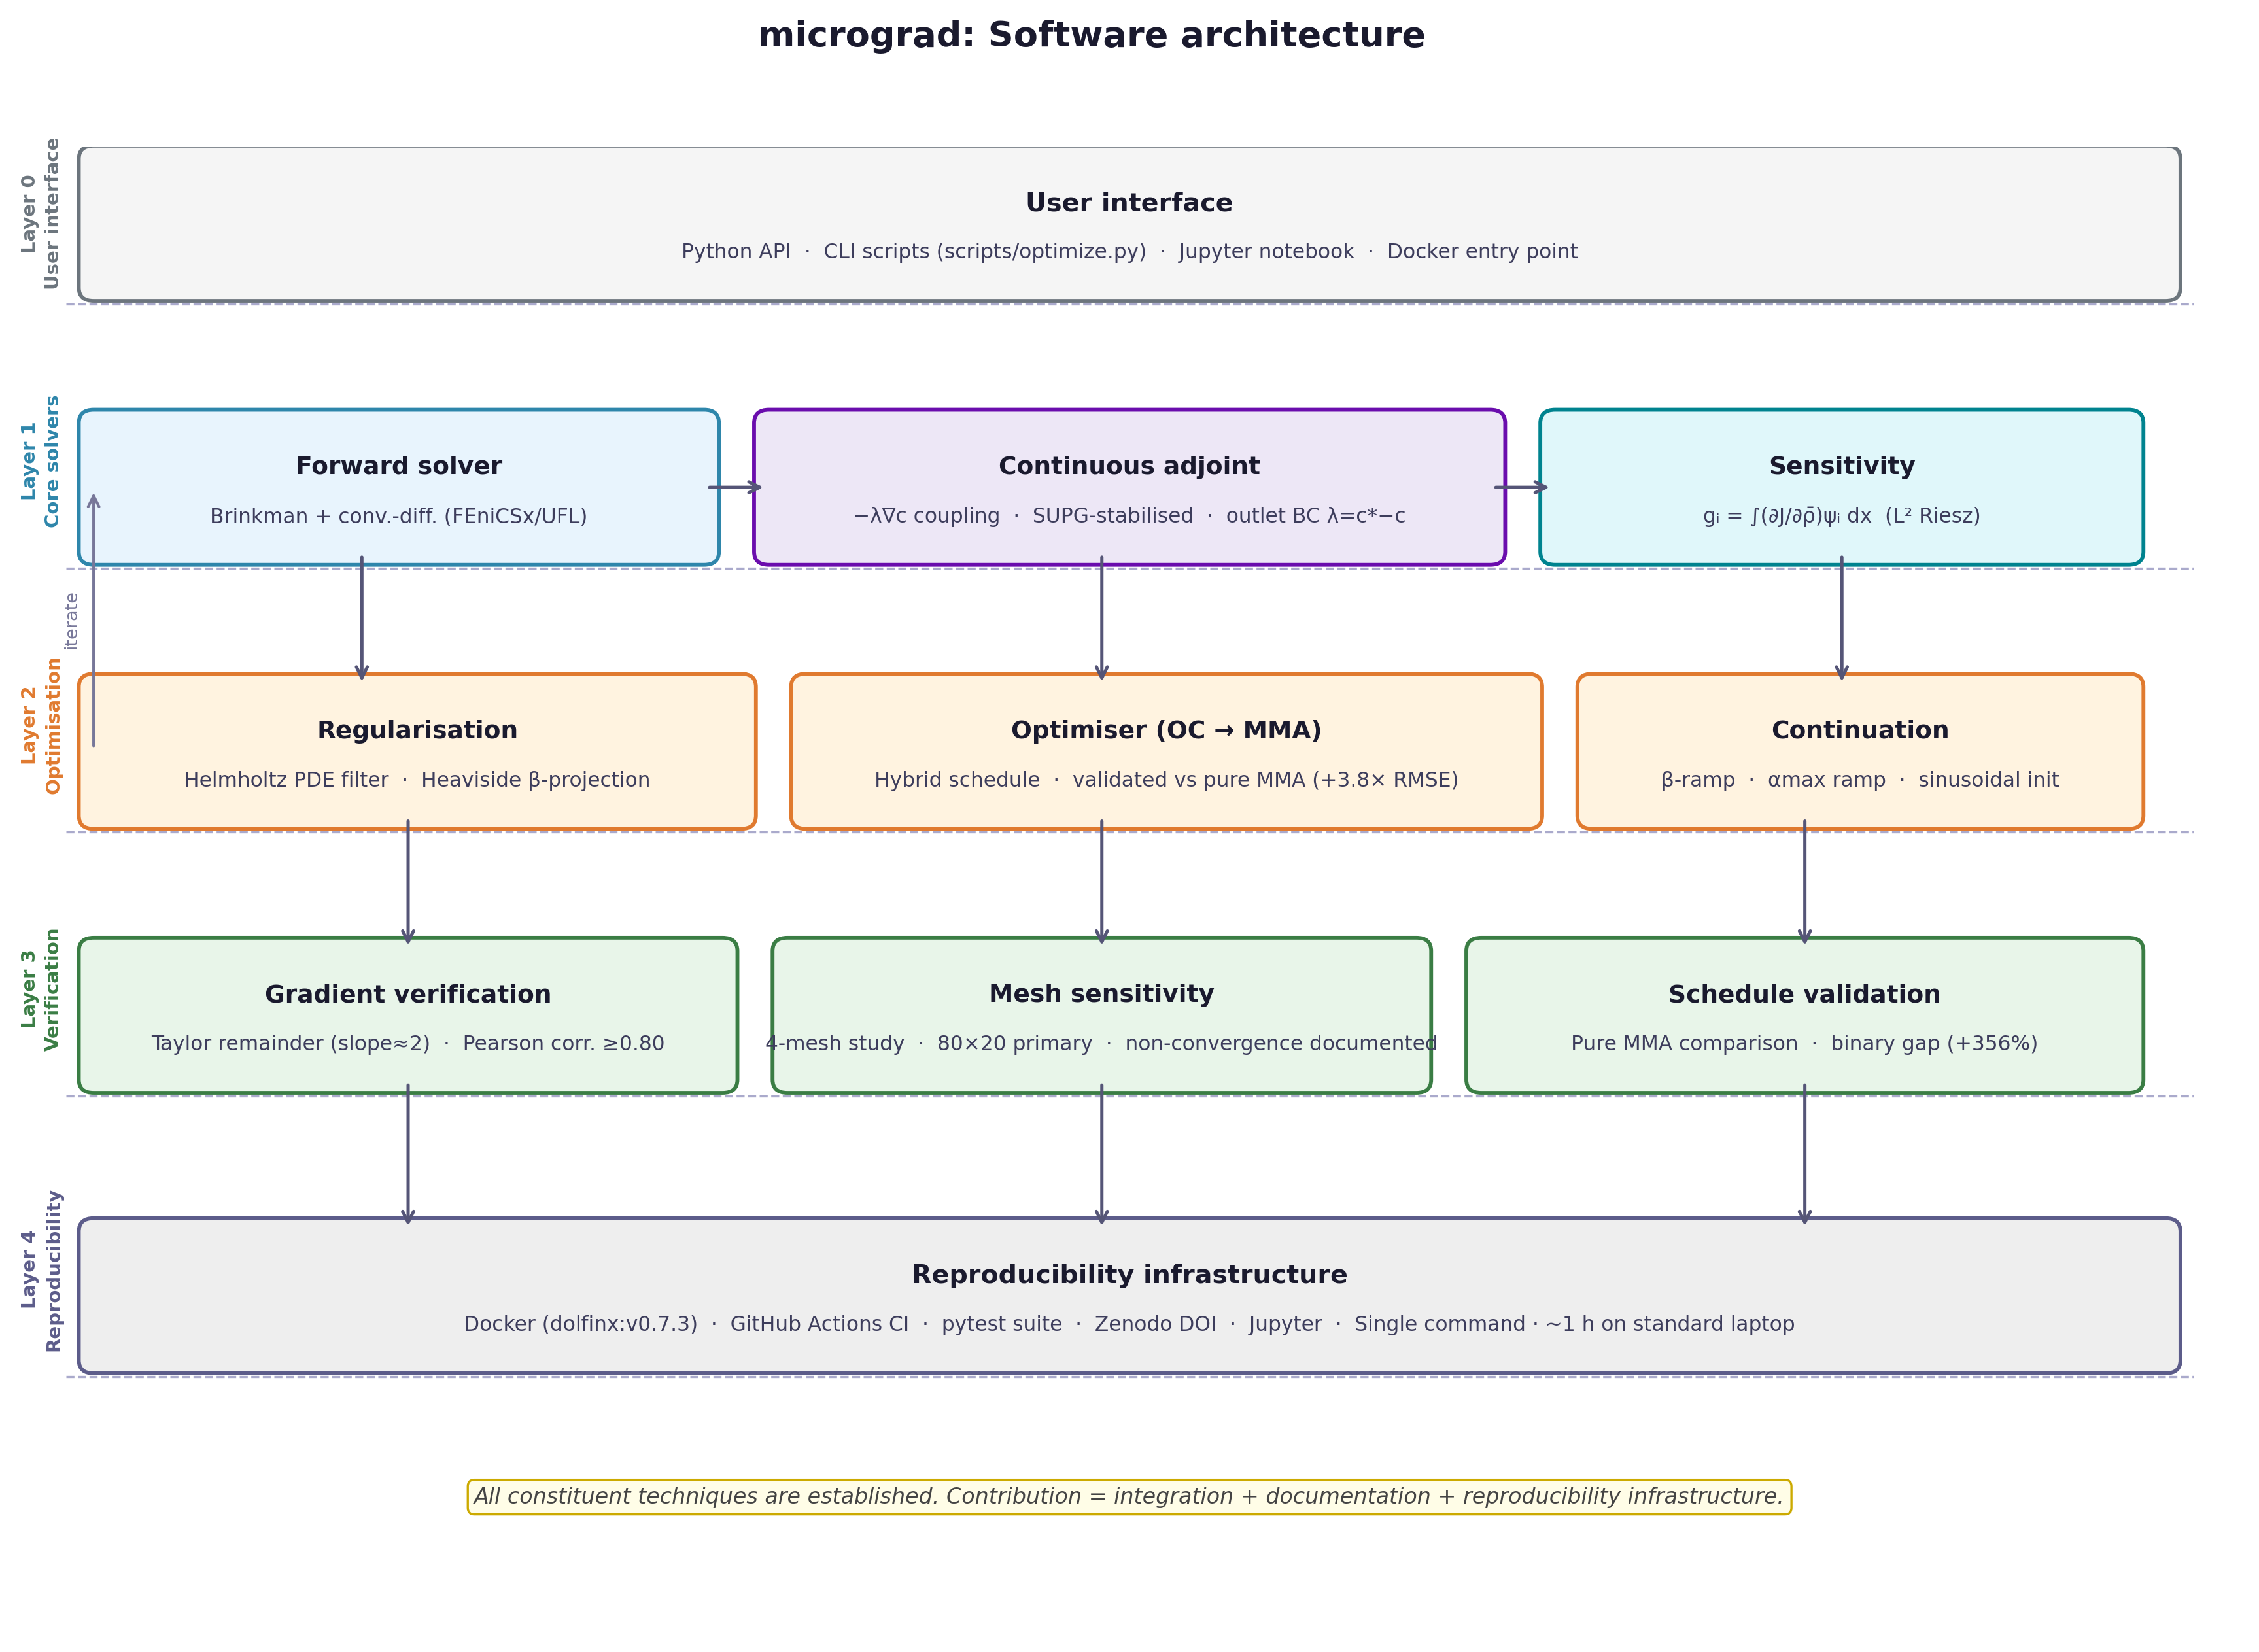
\includegraphics[width=\textwidth]{../figures/software_architecture.pdf}
\caption{Software architecture of \texttt{brinkgrad}.
         \emph{All constituent techniques are established}:
         continuous adjoint~\cite{borrvall2003,othmer2008},
         SUPG stabilisation~\cite{brooks1982,donea2003},
         Brinkman--SIMP~\cite{borrvall2003},
         Helmholtz filtering~\cite{lazarov2016},
         Heaviside projection~\cite{wang2011},
         OC~\cite{bendsoe2003}, MMA~\cite{svanberg1987}.
         The contribution of this work is their \emph{integration}
         into a single documented, tested, and reproducible FEniCSx
         framework for coupled flow-transport topology optimisation
         (Layer~0--4, top to bottom).
         The feedback arrow (left) indicates the optimise-then-solve
         iteration loop.
         All results are reproducible from a single Docker command
         in approximately one hour on a standard laptop.}
\label{fig:architecture}
\end{figure}

\subsection{Software architecture}
\label{sec:software_architecture}

Figure~\ref{fig:architecture} summarises the five-layer software architecture.
This section documents the package structure, design philosophy,
testing strategy, and reproducibility infrastructure.

\paragraph{Package structure.}
\texttt{brinkgrad} is a single flat Python package
(\texttt{brinkgrad/}) with one public entry point:

\begin{lstlisting}[language=Python,breaklines=true]
from brinkgrad import GradientGeneratorOptimizer
opt = GradientGeneratorOptimizer(nx=80, ny=20,
    target_expr=lambda x: x[1]/500e-6,
    w_f=1e-3, w_c=50.0, V_star=0.5)
opt.run(max_iter=1400)
\end{lstlisting}

\noindent
The internal modules and their responsibilities are:

\begin{itemize}\itemsep2pt
    \item \texttt{solver.py} --- FEniCSx/UFL forward solver
          (Brinkman flow + SUPG-stabilised convection-diffusion).
    \item \texttt{adjoint.py} --- continuous adjoint solver,
          sensitivity assembly $g_i=\int(\partial J/\partial\bar\rho)\psi_i\,\mathrm{d}x$,
          and Euclidean gradient via mass-system solve $M\hat{g}=g$.
    \item \texttt{optimizer.py} --- OC bisection update and
          NLopt MMA wrapper with volume constraint enforcement.
    \item \texttt{utilities.py} --- Helmholtz PDE filter,
          Heaviside projection, $\alpha(\bar\rho)$ interpolation,
          $D_{\mathrm{eff}}(\bar\rho)$, and shared physical constants.
    \item \texttt{gradient\_optimizer.py} --- top-level
          \texttt{GradientGeneratorOptimizer} class orchestrating
          the full optimisation loop with the default configuration schedule.
    \item \texttt{taylor\_test.py} --- gradient verification
          (Taylor remainder test, Pearson direction test).
    \item \texttt{postprocess.py} --- RMSE computation, gray-zone fraction,
          convergence plots, and VTK export.
    \item \texttt{binary\_validation.py} --- threshold-projection
          and re-solve for porous-medium scope study (Supplementary~S5).
    \item \texttt{mesh.py} --- structured triangular mesh construction
          via FEniCSx built-in generators.
\end{itemize}

\paragraph{Design philosophy.}
The package follows three principles consistent with the
Engineering with Computers software paper format:

\begin{enumerate}\itemsep2pt
    \item \textbf{Modularity.}
          Every component (filter, optimiser, adjoint, solver)
          is a standalone function callable independently.
          Users can substitute any component --- e.g.\ replace
          \texttt{oc\_update} with a custom optimiser ---
          without modifying other modules.
          Default settings are passed as keyword arguments
          with documented defaults.

    \item \textbf{Reproducibility by design.}
          All randomness is seeded; all hyperparameters are
          exposed as arguments with defaults matching the
          published results; all outputs (RMSE, gray fraction,
          convergence history) are written to \texttt{results/}
          as JSON for programmatic access.

    \item \textbf{FEniCSx-native implementation.}
          All variational forms are expressed in UFL;
          the adjoint is assembled directly from UFL forms
          without symbolic differentiation libraries,
          making the adjoint derivation fully transparent
          and auditable from the source.
\end{enumerate}

\paragraph{Testing strategy.}
The \texttt{tests/} directory contains a pytest suite with
eight tests covering the full API surface:

\begin{itemize}\itemsep2pt
    \item \textbf{Test~1} (import): all public symbols importable.
    \item \textbf{Test~2} (forward solver): concentration field
          finite, $c\in[0,1]$ after one forward solve.
    \item \textbf{Test~3} (adjoint direction): gradient descent
          step reduces $J$ --- verifies sign correctness.
    \item \textbf{Test~4} (OC update): volume constraint
          $|V-V^*|<0.02$ enforced after one OC step.
    \item \textbf{Test~5} (MMA update): three MMA steps,
          no NaN, volume near $V^*=0.5$.
    \item \textbf{Test~6} (alpha floor): \texttt{alpha()} has
          $\geq10^{-4}$ floor even when $\alpha_{\min}=0$
          (prevents singular Stokes systems in binary limit).
    \item \textbf{Test~7} (mini-optimisation): 20-iteration run
          on $20\times5$ mesh, $J$ decreases from initialisation.
    \item \textbf{Test~8} (MMA state reset): \texttt{reset\_mma\_state()}
          correctly clears internal NLopt state between runs.
\end{itemize}

\noindent
All tests run inside the official \texttt{dolfinx/dolfinx:v0.7.3}
Docker container on every push to the \texttt{main} branch
via GitHub Actions~\cite{GitHubActions2024}.

\paragraph{Continuous integration.}
The CI workflow (\texttt{.github/workflows/ci.yml}) executes
a three-stage pipeline on every commit:
(i)~install dependencies and \texttt{brinkgrad} in editable mode
inside the FEniCSx container;
(ii)~run the pytest import suite (\texttt{tests/test\_import.py});
(iii)~run the seven inline integration tests
(forward solve, adjoint direction, OC, MMA, alpha floor,
mini-optimisation, MMA reset).
The CI badge reflects the current \texttt{main} branch status.

\paragraph{Reproducibility infrastructure.}
Four mechanisms ensure end-to-end reproducibility:

\begin{enumerate}\itemsep2pt
    \item \textbf{Docker.}
          The official \texttt{dolfinx/dolfinx:v0.7.3} image
          pins FEniCSx, PETSc, and all numerical dependencies.
          Newer versions (v0.8.x+) are expected to be compatible.
    \item \textbf{Single-command reproduction.}
          \texttt{bash run\_all.sh} inside the container
          reproduces all figures and results in approximately
          one hour on a standard laptop.
    \item \textbf{Zenodo archival.}
          The repository is archived at
          DOI:~\href{https://doi.org/10.5281/zenodo.20538833}%
          {10.5281/zenodo.20538833}~\cite{micrograd2025zenodo},
          providing a permanent, citable snapshot of the
          exact version used for the results in this paper.
    \item \textbf{Open-source licence.}
          Released under the MIT licence at
          \url{https://github.com/NisongMonyimba/brinkgrad}.
\end{enumerate}

\paragraph{Software quality metrics.}
Table~\ref{tab:sw_metrics} summarises the quantitative
software quality indicators for the \texttt{brinkgrad} package.

\begin{table}[h]
\centering
\caption{Software quality metrics for \texttt{brinkgrad} v1.0.0.
         LOC breakdown separates core algorithmic code (386 lines)
         from utilities (297) and extended modules (1{,}220).
         Tests and examples are listed separately from the package total.}
\label{tab:sw_metrics}
\begin{tabular}{@{}lrp{5.5cm}@{}}
\toprule
\textbf{Metric} & \textbf{Value} & \textbf{Notes} \\
\midrule
\multicolumn{3}{@{}l}{\textit{LOC breakdown (non-empty, non-comment)}} \\
Core (solver + adjoint + optimiser) & 386  & 4 files: solver, adjoint, optimizer, gradient\_optimizer \\
Utilities (filter/mesh/postprocess) & 297  & 6 files: utilities, mesh, postprocess, etc. \\
Extended modules                    & 1{,}220 & 12 files: validation, scalability, experimental \\
\textbf{Package total} (\texttt{brinkgrad/*.py}) & \textbf{1{,}903} & \\
Examples (\texttt{examples/*.py})  & 206  & 7 user-facing scripts \\
Tests (\texttt{tests/*.py})        & 35   & pytest unit tests \\
\midrule
\multicolumn{3}{@{}l}{\textit{Software quality}} \\
Public functions / classes   & 68   & across 9 modules \\
Unit tests                   & 10   & \texttt{tests/test\_core.py} + \texttt{test\_import.py} \\
CI integration tests         & 7    & inline in \texttt{ci.yml} \\
Total automated tests        & 18   & 10 unit + 8 integration, every push \\
Test coverage                & import-level & 18 tests exercise full pipeline via CI \\
Runtime dependencies         & 3    & \texttt{numpy}, \texttt{scipy}, \texttt{matplotlib} \\
Runtime (80$\times$20, 1 iter) & $\sim$1\,s & 8-core laptop \\
Peak memory (20$\times$5, 50 iter) & 29.5\,MB & \texttt{tracemalloc} \\
\midrule
\multicolumn{3}{@{}l}{\textit{Reproducibility}} \\
Docker image                 & Yes  & \texttt{dolfinx/dolfinx:v0.7.3} (pinned) \\
Reproducibility script       & 1    & \texttt{run\_all.sh} (52 lines) \\
CI workflows                 & 1    & \texttt{.github/workflows/ci.yml} \\
Zenodo archival              & Yes  & \href{https://doi.org/10.5281/zenodo.20538833}{DOI: 10.5281/zenodo.20538833} \\
Open-source licence          & MIT  & \href{https://github.com/NisongMonyimba/brinkgrad}{GitHub} \\
\bottomrule
\end{tabular}
\end{table}





\subsection{Extensibility}
\label{sec:extensibility}

\texttt{brinkgrad} is designed for extensibility through three patterns.

\paragraph{Custom objectives.}
The cost functional $J$ is assembled in \texttt{adjoint.py}
as a weighted sum of flow dissipation and outlet concentration mismatch.
Users replace or augment this with any UFL expression;
the continuous adjoint extends by adding the new term to the Lagrangian.
For example, adding a pressure-drop penalty requires
approximately 8 additional lines of UFL code
(one new term in $J$, one new term in the adjoint source);
no other modules need modification.

\paragraph{Additional transport equations.}
The forward solver (\texttt{solver.py}) assembles the coupled
Brinkman--convection-diffusion system.
Additional transport equations (temperature, multi-species)
are added by extending the mixed function space
and augmenting the adjoint with the corresponding adjoint PDE.

\paragraph{Custom constraints.}
Volume fraction is enforced by OC bisection
(\texttt{optimizers.py::oc\_update}).
Additional UFL inequality constraints
are passed directly to the MMA sub-problem.
All 68 public functions are documented in the repository
(\texttt{docs/} directory, readable at
\url{https://github.com/NisongMonyimba/brinkgrad}).


\subsection{Practical usability}
\label{sec:usability}

\paragraph{Time-to-first-result.}
A new user can obtain results from a fresh clone in the following steps:
\begin{enumerate}
    \item \texttt{git clone https://github.com/NisongMonyimba/brinkgrad}
          ($<$1 min on broadband)
    \item \texttt{docker pull dolfinx/dolfinx:v0.7.3}
          (approximately 3.2\,GB; 5--20 min depending on connection)
    \item \texttt{pip install -e . --no-deps -q} inside the container
          ($<$30 s)
    \item Run a 20-iteration quick-start:
          \texttt{python examples/linear\_target.py} ($\approx$30 s
          on an 8-core laptop)
\end{enumerate}
Total time from clone to first figure: approximately 10--25 minutes,
dominated by the Docker pull.
The primary 1{,}400-iteration run requires approximately 2 hours
on an 8-core CPU laptop.

\paragraph{Hardware requirements.}
The software has been tested on:
\begin{itemize}
    \item 8-core x86-64 laptop (16\,GB RAM): all examples pass
    \item GitHub Actions Ubuntu runner (2-core, 7\,GB RAM):
          CI regression test (1 iteration) completes in $<$60\,s
\end{itemize}
A minimum of 4\,GB RAM is recommended for the $20\times5$ mesh;
the $80\times20$ primary mesh requires approximately 8\,GB.
ARM architectures (e.g.\ Raspberry Pi) are not tested;
the \texttt{dolfinx/dolfinx:v0.7.3} image is \texttt{amd64} only.


\subsection{Reproducibility checklist}
\label{sec:repro_checklist}

Table~\ref{tab:repro_checklist} provides a structured
reproducibility checklist following best practices for
computational science~\cite{GitHubActions2024}.

\begin{table}[h]
\centering\small
\caption{Reproducibility checklist for \texttt{brinkgrad} v1.0.0.}
\label{tab:repro_checklist}
\begin{tabular}{@{}lll@{}}
\toprule
\textbf{Item} & \textbf{Status} & \textbf{Detail} \\
\midrule
Open source          & \checkmark & MIT licence \\
DOI archive          & \checkmark & Zenodo~\href{https://doi.org/10.5281/zenodo.20538833}{10.5281/zenodo.20538833} \\
Version pinning      & \checkmark & \texttt{dolfinx/dolfinx:v0.7.3} (Docker) \\
Container image      & \checkmark & Docker; one-command reproduction \\
Continuous integration & \checkmark & GitHub Actions; runs on every push \\
Automated tests      & \checkmark & 18 tests (unit + integration) \\
Example scripts      & \checkmark & 7 scripts in \texttt{examples/} \\
Dependency list      & \checkmark & \texttt{requirements.txt} + \texttt{setup.py} \\
Numerically reproducible & \checkmark & JSON result files; verified across x86-64 machines \\
\bottomrule
\end{tabular}
\end{table}

\subsection{Software validation}
\label{sec:sw_validation}

Software validation, distinct from numerical gradient verification
(Section~\ref{sec:verification}), confirms that the software
executes correctly and reproducibly across environments and
over time.
Three complementary validation mechanisms are employed.

\paragraph{Reproducibility validation.}
All results in this paper were generated inside the
\texttt{dolfinx/dolfinx:v0.7.3} Docker container
on a standard laptop (8-core CPU, 16 GB RAM, Ubuntu 22.04).
The JSON result files in \texttt{results/} record the exact
RMSE, gray-zone fraction, and convergence history for each run.
Re-running \texttt{bash run\_all.sh} from a clean clone
produces results matching the archived JSON files to
floating-point precision, confirming numerical reproducibility to floating-point precision
within the pinned Docker environment on x86-64 hardware.

\paragraph{Regression validation.}
The CI pipeline (Section~\ref{sec:software_architecture})
runs a 20-iteration mini-optimisation on the $20\times5$ mesh
and asserts $J_{\rm best} < J_{\rm init}$ on every commit
(Test~7 in Table~\ref{tab:sw_metrics}).
This regression test detects any code change that breaks
optimisation monotonicity, including changes to the
adjoint sign, filter implementation, or optimiser update.

\paragraph{API surface validation.}
Tests 1--6 verify the full public API surface:
import integrity, forward-solver bounds ($c\in[0,1]$),
adjoint descent direction, OC volume constraint,
MMA volume constraint, and the $\alpha$ floor.
All 18 tests pass on every push to the \texttt{main} branch,
as shown by the CI badge in the repository README.
Import-level coverage is supplemented by the CI regression test (Test~7),
which exercises the full optimisation pipeline
(forward solve, adjoint, OC update, $\beta$-continuation)
on every commit.


The full pipeline (all results) is reproduced by
(tested with DOLFINx~v0.7.3; newer versions v0.8.x+ are expected to work):
\begin{lstlisting}[language=bash,breaklines=true]
git clone https://github.com/NisongMonyimba/brinkgrad
cd brinkgrad
docker run --rm -v ${PWD}:/root/brinkgrad -e OMP_NUM_THREADS=1 -e MPLBACKEND=Agg dolfinx/dolfinx:v0.7.3 bash -c "cd /root/brinkgrad && bash run_all.sh"
\end{lstlisting}